% TODO:
% Sentence to introduce the results section.
We evaluate the extent to which diffusion MRI microstructural features enable robust prediction of 
demographic and clinical variables across model families, feature representations, and cross-validation 
folds. Beyond absolute performance, we explicitly analyze performance variability to assess the stability 
and generalizability of different configurations.
% Is it possible to predict information/demographics from diffusion MRI microstructure? Several papers have 
% proposed methods to do so, but it remains unclear which models and feature representations are best suited for this task.
% Predictions across different datasets and microstructure representations show a huge variability as shown in
% \ref{fig:model_family}. How can we ensure that the prediction we performed with a model is going to become
% a robust and generalizable method when the prediction with a different configuration microstructure-model is lower? 

\begin{figure}
    \centering
    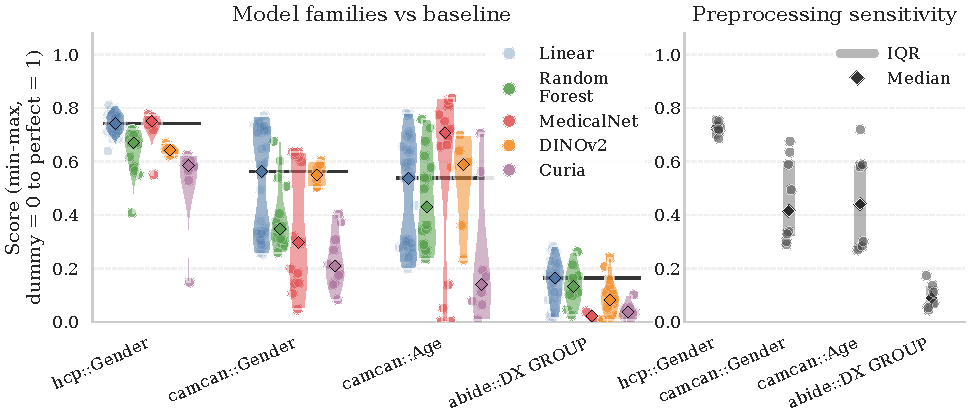
\includegraphics[width=\textwidth]{../exp_outputs/summary/plots/folds/combined_model_vs_prep.png}
    \caption{Summary of benchmark results across datasets, feature representations and models.}
    \label{fig:model_family}
\end{figure}

Figure \ref{fig:model_family}  reveals two important patterns. First, regularized linear models consistently 
perform on par with deep learning approaches, despite their lower representational capacity. While deep 
architectures achieve competitive performance, the gap between model families is often smaller than expected,
suggesting that microstructural feature representation may be as critical as model complexity. Second, and more remarkably, 
we observe substantial variance in prediction performance across models and microstructural 
parameterizations. In several settings, this variability exceeds \textbf{the mean difference between model families}, 
indicating that conclusions drawn from a single model or microstructural representation may be unstable. These findings 
underscore the importance of reporting variability and evaluating robustness across configurations when 
assessing predictive performance in diffusion MRI.


\begin{figure}
    \centering
    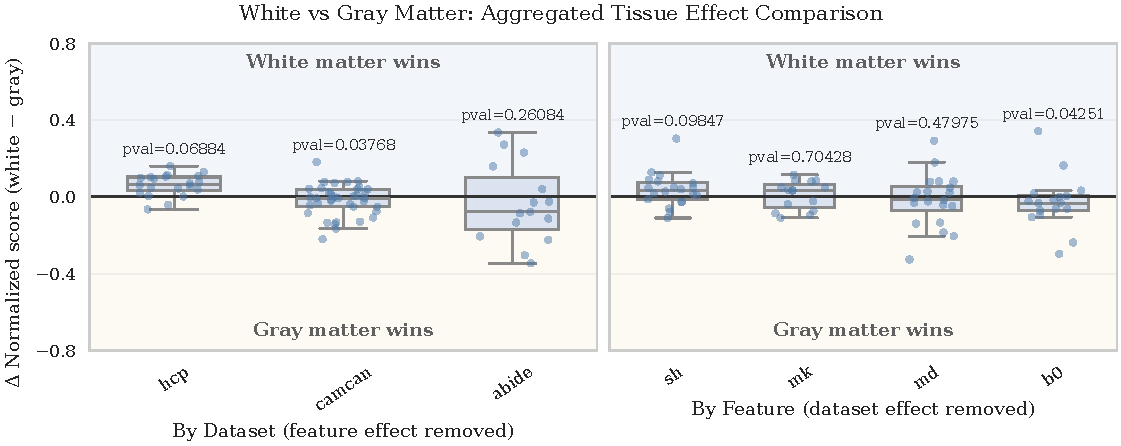
\includegraphics[width=\textwidth]{../exp_outputs/summary/plots/folds/white_vs_gray_tscore_dataset_feature_combined.png}
    \caption{Comparison of white vs gray matter performance across d
    atasets and feature representations.}
    \label{fig:white_vs_gray}
\end{figure}
% TODO: \autoref{fig:white_vs_gray} Variability across tissue types

% In general, when studies predict demographic or clinical variables from diffusion MRI, they often focus on a 
% single tissue type (e.g., white matter) and a specific set of microstructural features. However, our results 
% suggest that the choice of tissue type and microstructural representation can have a significant impact on 
% predictive performance.

% Analyzing another level of extraction and going into thebrain specifics of tissue and microstructural feature 
% representation, we can see in 
% \ref{fig:white_vs_gray} that for the same dataset and model configuration, the choice of microstructural 
% features has a significant impact on prediction performance, and not only the microstructural features but 
% the tissue type from where we extract the information. 
% We conduct the task predictions with both tissue types (gray and white matter) to evaluate the predictive imapact according
% to the tissue type according to different microstructural features and datasets. We observe that, in general, 
% gray matter features tend to outperform white matter features across datasets and tasks, suggesting that gray 
% matter microstructure may carry more predictive information for demographic and clinical variables (or maybe its 
% representation was more informative). The variability in performance across feature representations and tissue 
% types further emphasizes the need for comprehensive evaluation to identify robust predictors in diffusion MRI.

We further isolate the effect of tissue compartment by performing paired, fold-level 
comparisons between the best-performing gray and white matter models within each 
dataset–target–task–feature configuration. Rather than comparing raw averages, we compute a 
standardized paired difference that accounts for fold variability, thereby estimating a 
tissue-specific effect size. As shown in Figure \ref{fig:white_vs_gray}, the direction and 
magnitude of this effect depend strongly on both dataset and microstructural representation.

When aggregated across independent configurations, we observe that the magnitude effect is 
often comparable to the variability observed across folds, underscoring 
that tissue choice constitutes a non-negligible design decision. These results suggest 
that restricting analyses to a single compartment may overlook informative microstructural 
signals and lead to configuration-dependent conclusions.


\begin{figure}
    \centering
    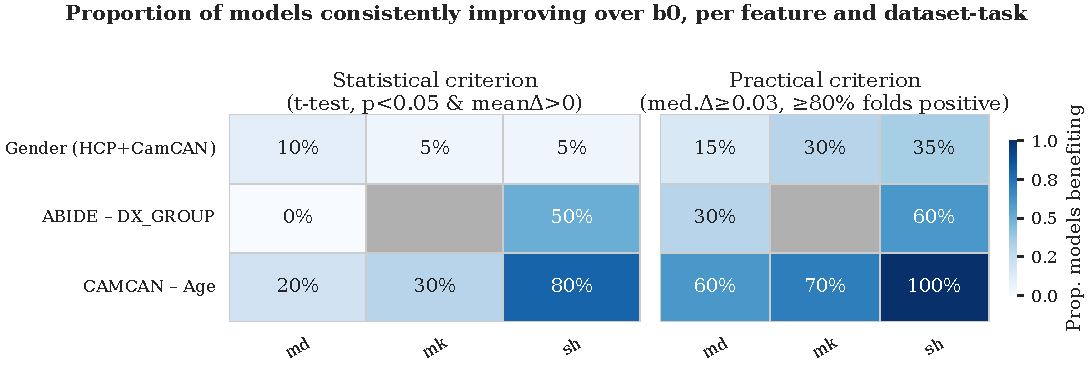
\includegraphics[width=\textwidth]{../exp_outputs/summary/plots/features/feature_benefit_heatmap.png}
    \caption{Impact of different feature representations on prediction performance across datasets and tasks.}
    \label{fig:feature_impact}
\end{figure}

% \subsection{Within-Dataset Performance}
% \begin{itemize}
%     \item Model/Feature/Tissue comparison
%     \item Mean ± std of best run / model
%     \item Statistical testing
%     \item PLOT: Bar plots per dataset | Camcan-HCP comparison(?
% \end{itemize}

% \subsection{Feature Representation Comparison}
% \begin{itemize}
%     \item Gray vs white matter
%     \item Microstructure metrics comparison
%     \item PLOT: Tissue performance according to microostructure metric for task purposes | Microstructure features
% \end{itemize}

% \subsection{"Handmade" vs DL embeddings}

% \subsection{Training Size Analysis}
% * PLOT: Learning Curve

% \subsection{Key Findings}
% \begin{itemize}
%     \item Which models perform best? Which feature representations perform best? Tissue predominance in task prediction?
%     \item Are simpler models sufficient? Are DL models necessary for predicting demographics?
%     \item Stability across folds?
% \end{itemize}

% \subsection{Methodological Insights}
% \begin{itemize}
%     \item Importance of dimensionality control
%     \item Effect of tract-based aggregation 
%     \item Risk of overfitting in mesh representations without PCA bcs of the high number of vertices representations
% \end{itemize}